\documentclass[10pt,a4paper]{article}

\usepackage[utf8]{inputenc}
\usepackage[english,russian]{babel}
\usepackage{amsmath}
\usepackage{amsfonts}
\usepackage{amssymb}
\usepackage{textcomp}
\usepackage{graphicx}
\usepackage{hyperref}
\usepackage{fancyvrb}

\usepackage[margin=17mm]{geometry}

\begin{document}

\title{Скрытые Марковские модели переменного порядка для анализа данных
  ChIP-seq}
\author{Атаманова Анна, кафедра системного программирования СПбГУ, \url{anne.atamanova@gmail.com}}

\maketitle

\begin{abstract}
  Здесь нужно кратко описать суть работы и результаты.
\end{abstract}

\section{Введение}

ДНК (дезоксирибонуклеиновая кислота) --- длинная двухцепочечная молекула, являющаяся носителем
генетической информации в биологических организмах. В клетках эукариот ДНК
находится в упакованном состоянии. Упаковка ДНК реализована с участием
специальных белковых комплексов --- нуклеосом. Химические модификации субъединиц
нуклеосомы, гистонов, могут влиять на плотность упаковки ДНК. Увеличение
плотности ДНК влияет на доступность соответствующих участков ДНК для внутренней
машинерии клетки.

%% TODO: чуть больше информации о важности изучения химических модификаций
%% хвостов гистонов

Иммунопреципитация хроматина с последующим секвенированием (chromatin
immunoprecipitation sequencing, ChIP-seq) --- это биологический протокол,
позволяющий получить информацию о наличие или отсутствии некоторой химической
модификации гистонов вдоль генома \cite{Johnson2007}. Суть метода заключается в
использовании антитела для отбора фрагментов ДНК, cвязанных с гистонами,
имеющими изучаемую химическую модификацию с последующим секвенированием. В ходе
секвенирования случайные фрагменты ДНК, читаются секвенатором в объёме,
достаточном для того, чтобы с большой вероятностью каждый фрагмент был прочитан
несколько раз. Затем для каждого полученного прочтения ищется соответствующий
ему участок последовательности генома (рис.~\ref{fig:chip-seq}). Обычно
прочтения, которым может соответствовать более одного участка в геноме,
исключают из рассмотрения.

\begin{figure}[h]
  \centering
\begin{Verbatim}[commandchars=\\\{\}]
          CAAAAGACAAATAGTGATGTCACCAATCGAGC
          --------------------------------
               GACA ATA     GTCA   AATG
              AGAC   TAGTG TGTC
               GACA   AGTG TGTCA   ATCG

          00001100001110000110000001000000
\end{Verbatim}
  \caption{Схематическое изображение выравнивания прочтений секвенатора (под чертой)
    на известную последовательность генома (над чертой).}
  \label{fig:chip-seq}
\end{figure}

Результаты эксперимента представляют в виде вектора длины генома, в котором
стоит 1, если в соответствующей позиции генома начинается хотя бы одно прочтение
и 0 в обратном случае.

%% TODO: описать разбиение на бины и ввести обозначения.

Протокол хроматин-иммунопреципитации, как и большинство биологических
протоколов, не исключает наличие в результатах эксперимента
ошибок. Недостаточная специфичность антитела, наличие ошибок секвенирования
и нестабильность положения гистонов на ДНК приводят к возникновению сигнала не
зависящего от наличия изучаемой модификации гистонов. Использование
вероятностных моделей позволяет провести анализ результатов
хроматин-иммунопреципитации с учётом наличия ошибок.

Большинство существующих моделей (TODO: ref) для данных
хроматин-иммунопреципитации основано на аппарате скрытых Марковских моделей
второго порядка с Пуассоновскими испусаниями. Использование распределения
Пуассона для покрытия, опирается на предположение о том, что в каждой
позиции генома в среднем начинается одинаковое количество прочтений. Марковский
процесс, как правило, имеет два состояния $+$ --- сигнал есть и $-$ --- сигнала
нет. Второй порядок модели означает, что состояние некторого окна зависит только
от состояния его прямого предшественника.

Использование моделей второго порядка объясняется тем, что количество параметров
модели, а также сложность её обучения и использования экспоненциально зависят от
порядка, то есть, модель порядка $m$ требует оценки $2^m$ параметров.

%% TODO: четче объяснить привлекательность модели второго порядка и перейти к
%% цели работы.

В настоящее время, в качестве семейства искомых моделей, активное приминение находит HMM (Hidden Markov Model)\cite{Rabiner1989} второго порядка с Пуассоновским испусканием.
Данное семейство допускает предположение о том, что каждое состояние (наличие/отсутствие белка в заданной части генома) завист только от одного предыдущего.
Можно ограничиться и более лояльным допущением о том, что состояние зависит от $n$ предыдущих состояний, однако такое допущение резко увеличивает сложность модели ($O(2\textsuperscript{n})$ параметров). Также, сложность заключается в подборе этого $n$ и переобучении в случае, если не все состояния имеют одинаковые длины контекстов зависимости.
Последннее замечание подводит к идее использования VOHMM (Variable Order Hidden Markov Model)\cite{Wang2006}


\section{Скрытые марковские модели переменного порядка}

Марковский процесс порядка $ m $ - это случайный процесс, эволюция которого в каждый момент времени зависит только от $ m-1 $ предыдущих состояний.

Другими словами, $ X = (x_{1}, x_{1}, ..., x_{T}) $ является марковской цепью порядка $ m $,
если $ p(x_{t}|x_{1}^{t-1}) = p(x_{t}|x_{t-m+1}^{t-1})$

Таким образом, каждое следующее состояние определяется контекстом длины $ m-1 $ и вероятностями перехода из него.

Скрытая марковская модель предполагает, что, помимо всего прочего, каждое состояние задает свою вероятностною модель (например, гауссиан), а в качестве наблюдений поступают не сами состояния, а лишь испускания из них $y_{1},...,y_{T}$ (\ref{ris:image}- пример HMM порядка 2).
\begin{figure}[hbtp]
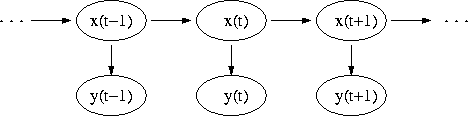
\includegraphics[scale=0.4]{Hmm_temporal_bayesian_net.png}
\centering
\caption{HMM order 2}
\label{ris:image}
\end{figure}


Скрытая марковская модель переменного порядка - обобщение HMM разрешающее иметь контекстам разные длины.

Итого, скрытая марковская модель переменного порядка определяется контекстами, вероятностными распределениями переходов и верояностными распределениями испусканий для каждого состояния.

Перейдем к обучению модели по цепочке наблюдений.

Обычно обучение $ n-hmm$ $ m $-го порядка сводится к $ n^{m}-hmm второго порядка$, котрая обучается алгоритмом Баума-Велха (частный случай EM алгоритма, который итеративно максимизирует правдоподобие модели).

Для хранения контекстов используется дерево (бор), в котором вершины являются строками, ребра буквами. Корень - это пустой контекст, а каждый ребенок вершины является уточнением контекста родителя на состояние ребра.
Итого, каждая внутренняя вершина имеет ровно n потомков. Листья - главные контексты.

Заметим, что, если дети какой-то вершины имеют одинаковые вероятности переходов, то они контекст вершины не уточняют, и их можно обрезать.

Так же заметим, что достаточно хранить только листья и распределение переходов на них, и, в случае необходимости, пересчитывать его на внутренние вершины

$ p(q|s) = \frac{\sum_{c \in C(s)} {p(q|c)}}{\sum_q\sum_{c \in C(s)} {p(q|c)}} $ ,

где $ q $ - состояние, $ C(s )$ - все листья (контексты), являющися потомками $ s $

Изначально берется полное дерево некоторой фиксированной глубины $m$.

Обучение модели по цепочки наблюдений происходит с помощью чередования EM-алгоритма и обрезания дерева.

EM-часть максимизирует правдоподобие модели алгоритмом Баума-Велха

Обрезание дерева производится нахождением родителей лиистьев, все потомки которых имеют близкие распределения переходов. Все дети такой вершины ликвидируются, а сама вершина становится новым контекстом. Критерием сравнения распределений переходов служит расстояние Кульбака-Лейблера.

Инициализация каждого следующего EM ведется с помощью пересчета распределения переходов на новые контексты.

Изначальная инициализация производится путем построения цепочки состояний алгоритмом $ k $-means по наблюдениям (где $k=n$) и частотной оценкой вероятности переходов на ней.

\section{Оценка модели}

\section{Заключение}

\bibliographystyle{plain}
\bibliography{references}

\end{document}
